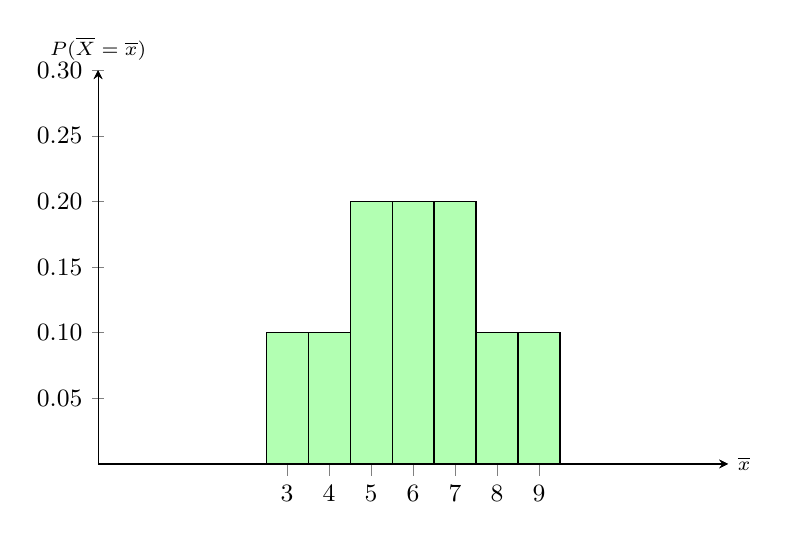
\begin{tikzpicture}
  \begin{axis}[
      scale only axis,
      axis lines=left,
      no markers,
      xmin = -1.5, xmax = 13.5,
      ymin = 0, ymax = 0.3,
      samples at={3,4,8,9},
      xtick={3,4,8,9},
      ytick={0.05,0.1,...,0.3},
      y tick label style={
        /pgf/number format/.cd,
        fixed,
        fixed zerofill,
        precision=2,
        /tikz/.cd
      },
      ticklabel style={font=\small},
      enlargelimits=false,
      clip=false,
      axis on top,
      grid = none,
      ybar=0pt, 
      bar width=1,
      height=5cm,
      width=8cm
    ]
    \addplot [fill=green!30] {0.1};
    \node [right] at (axis description cs: 1,0) {\scriptsize $\overline x$};
    \node [above] at (axis description cs: 0,1) {\scriptsize $P(\overline X = \overline x)$};
  \end{axis}

  \begin{axis}[
      scale only axis,
      axis lines=left,
      no markers,
      xmin = -1.5, xmax = 13.5,
      ymin = 0, ymax = 0.3,
      samples at={5,6,7},
      xtick={5,6,7},
      ytick=\empty,
      ticklabel style={font=\small},
      enlargelimits=false,
      clip=false,
      axis on top,
      grid = none,
      ybar=0pt, 
      bar width=1,
      height=5cm,
      width=8cm
    ]
    \addplot [fill=green!30] {0.2};
  \end{axis}

\end{tikzpicture}